Any Berkovich analytification $X\an$ of a smooth connected proper curve can be decomposed into two types of $K$-analytic spaces, \emph{Berkovich balls} and \emph{annuli}.
In fact these decompositions in such pieces are in correspondence with the semi-stable formal models of $X\an$. 
In this section based on \cite[sec.\ 2]{bakerStructureNonarchimedeanAnalytic2013} will define these  
Hence its worth to discuss these objects. 
These can be described as affinoid domains in $\aff^{1}\an$, which is handy because we've discussed $\aff^{1}\an$ in quite some detail already.  
\begin{figure}[h]
	\centering
	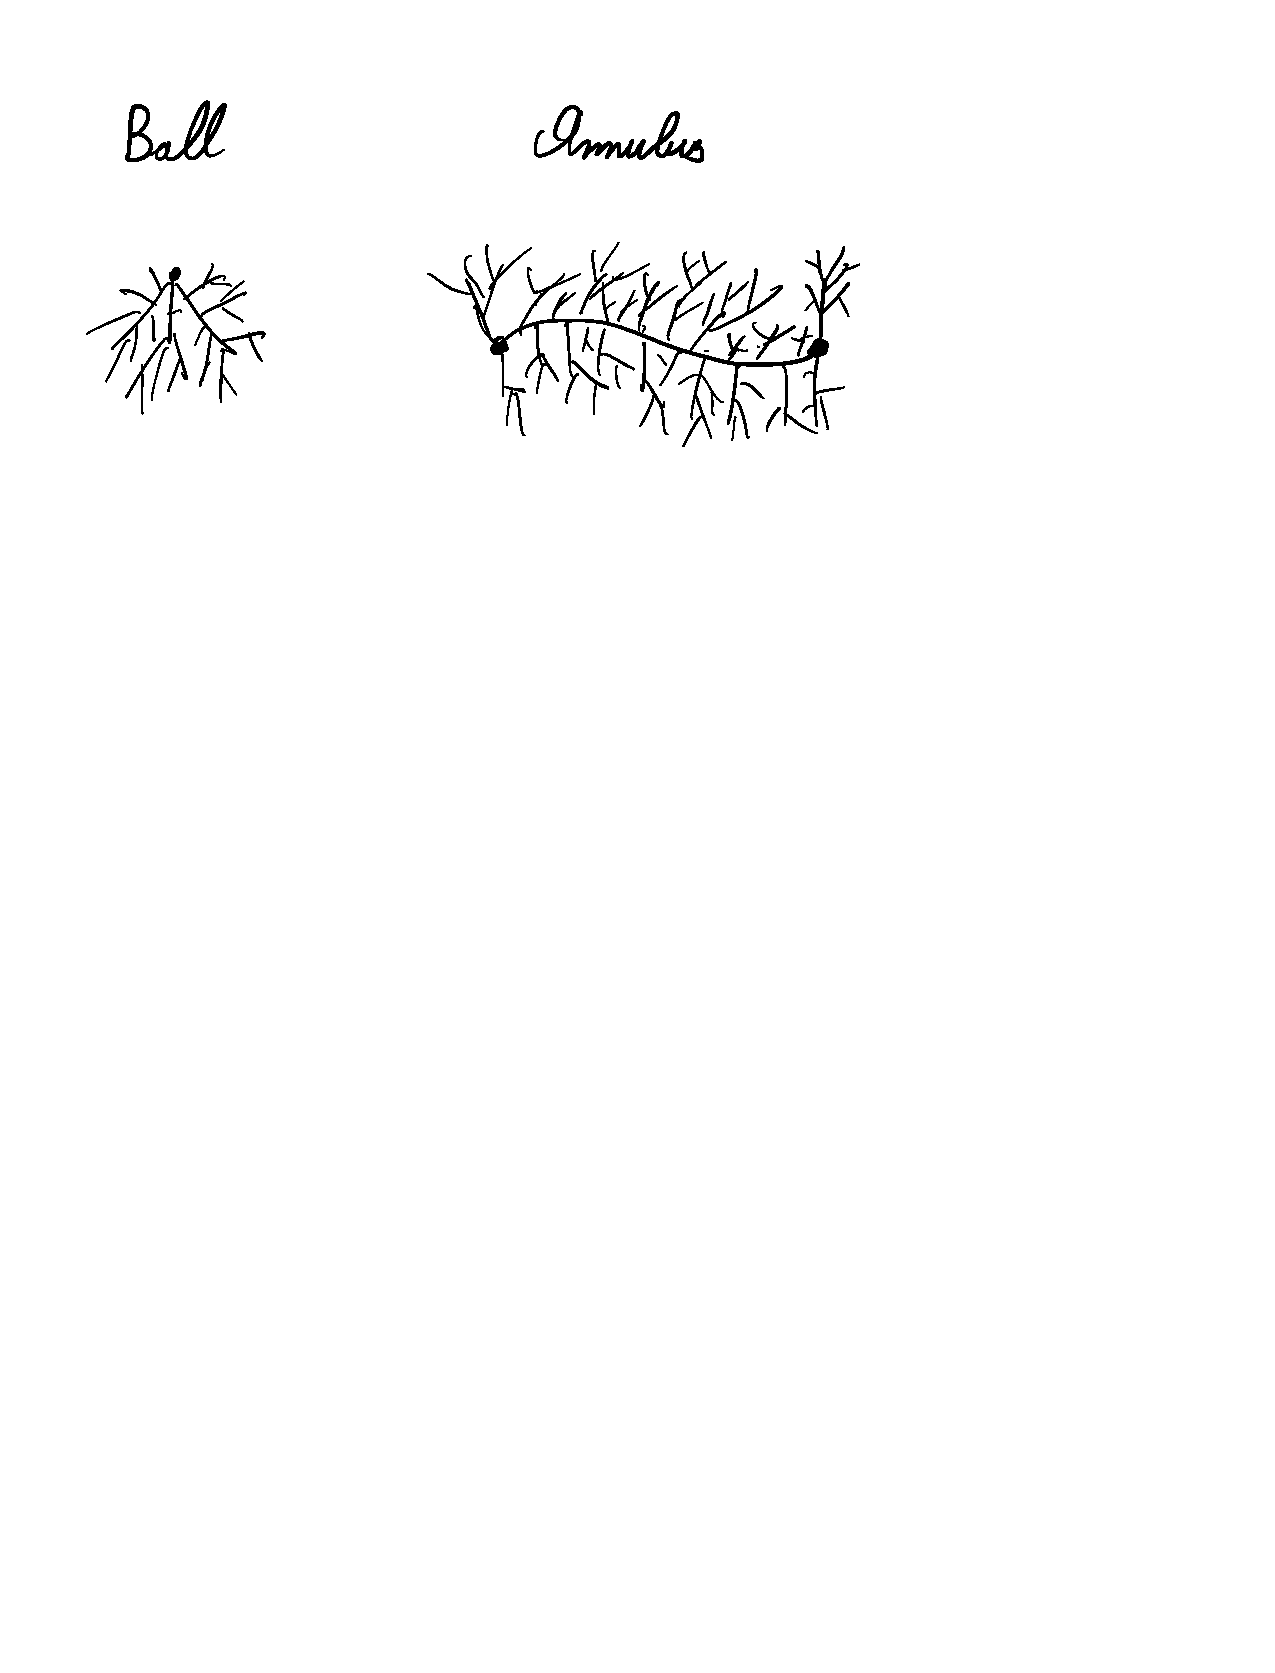
\includegraphics[width=0.6\textwidth]{figures/ball_annulus}
	\caption{A Berkovich ball and Annulus}
	\label{fig:ball_annulus}
\end{figure}
\begin{definition}
	The \emph{tropicalisation map} is the map 
	\begin{align*}
		\trop :  \mathcal{M} (K[T]) &\longrightarrow \R \cup \{\infty\}  \\
		x &\longmapsto -\log( \|T\|_x)
	.\end{align*}
	Here $\mathcal{M} (K[T])$ is the Berkovich affine line and equals $\aff^{1}_K\an$. 
\end{definition}
Intuitively you should think of this map as giving the inverse logarithmic distance from the origin of $\aff^{1}\an$ on the line $\ell_0$ (recall \cref{eq:line_in_A_1}).  
The whole of $\aff^{1}\an $ retracts on this line, and takes the value of the point where it contracts to. Hence off the line $\ell_0$ the function $\trop$ is locally constant. 



\begin{definition}
	Let $r \in |K^{\times }|$. The \emph{standard closed ball} of radius $r$ is $B(r) = \trop^{-1}([-\log r, \infty])$, i.e. $B(a) = \{x \in \aff^{1}\an \st \|T\|_x \le r\} $. 
\end{definition}
The standard closed ball is also the Berkovich spectrum of the Tate algebra \[
K\left<r^{-1}t \right> = \left\{\sum_{n = 0}^{\infty} a_n ^{n} \st r ^{n} \|a_n\| \to 0 \text{ as } n \to \infty \right\} 
.\] 
\begin{definition}
	Again let $a \in |K^{\times }|$. 
	The \emph{standard open ball} of radius $r$ is $B(a)_+ = \trop^{-1}((-\log r, \infty])$, i.e.\ $B(a) = \{x \in \aff^{1}\an \st \|T\|_x <  r\} $.
\end{definition}

\begin{definition}
	Let $r, s \in |K^{\times }|$. 
	The \emph{standard closed annulus with outer radius  $r$ and inner radius  $s$}  is $S(s, r) = \trop^{-1}([-\log r, -\log s])$, i.e.\ $S(s, r) = \{x \in \aff^{1}\an \st s \le \|T\|_x \le r\} $.

	The \emph{modulus} of this annulus is $s r^{-1}$. 
\end{definition}
The standard closed annulus is also the Berkovich spectrum of the affinoid algebra \[
	K\left<r^{-1}t, st^{-1} \right> = \left\{\sum_{n \in \Z}^{} a_n ^{n} \st r^{n}|a_n| \to 0 \text{ as } n \to +\infty, s^n |a_n| \to 0 \text{ as } n \to - \infty\right\} 
.\] 
If $r = 1$ then we write $S(s) = S(s,1)$. 
\begin{definition}
	Again take $r, s \in |K^{\times }|$. 
	The \emph{standard open annulus of outer radius $r$ and inner radious $s$} is $S(s,r)_+ = \trop^{-1}((-\log s, -\log r))$. 
	I.e.\ $S(s,r)_+ = \{x \in \aff^{1}\an \st s < \|T\|_x < r\} $

	Similarly to the closed annulus we define the \emph{modulus} of this ball to be $s r^{-1}$. 
\end{definition}

\begin{figure}[ht]
    \centering
    \incfig{affine-line-ball-annuli}
    \caption{Balls and annuli as domains in $\aff^{1, \text{an}}_K$}
    \label{fig:affine-line-ball-annuli}
\end{figure}

Finally we define a domain that is not quite an annulus as defined above, but is very similar to one. 
\begin{definition}
	Let $r \in |K^{\times }|$. The \emph{standard punctured open ball of radius $r$ } is $S(0, a)_+ = \trop^{-1}((-\log a, \infty))$. 
	The \emph{standard punctured open ball of radious $r^{-1}$ around $\infty$} is $S(a, \infty)_+ = \trop^{-1}((-\infty, -\log a))$. 

	By definition we say these are annuli of modulus $\infty$. 
\end{definition}

All closed balls with $r \in |K^{\times }|$ are isomorphic. Similarly all open balls with $r \in |K^{\times }|$ are isomorphic. 
Two open (resp.\ closed) annuli/punctured balls are isomorphic if and only if they have the same modulus. 

\begin{remark}
	If we just remove $0$ from $\aff^{1}\an$ (and thus also $\infty$ of $\pro^{1}\an$) we gain obtain something similar to an annulus. But the outer radius is $\infty$ and the inner radius is $0$. 
	Note that this is also $\mathbb G^{\mathrm{an}}_m$, which how we will usually denote this space. 
\end{remark}


Note that annuli have a special line running between two boundary points, where all the rest of the annulus branches of from. This line is called the \emph{skeleton} and it is not just an artefact of how we decided to draw the annulus, as it can be described in the following way. 
\begin{proposition}[prop.\ 2.2.5 in \cite{thuillierTheoriePotentielCourbes2005}]
	The skeleton of a annulus are exactly the points that lay not an affinoid isomorphic to a closed ball.  
\end{proposition}

The notion of a skeleton can be extended to the analytification of any curve, and these skeleta will be crucial in the study of curves and their models. 

